\documentclass{article}
\usepackage[polish]{babel}
\usepackage[T1]{fontenc}
\usepackage[utf8]{inputenc}
\usepackage{graphicx}

\title{Sprawozdanie Programowanie Komponentowe}
\author{Kacper Ochnik}
\date{\today}

\begin{document}

\maketitle

\newpage
\section*{1. Opis Zadania Programistycznego}

Niniejsze sprawozdanie opisuje implementację aplikacji komponentowej w języku Java.
Aplikacja komponentowa powinna składać się z komponentów które:
\begin{itemize}
    \item posiadają dane i metody operujące na tych danych
    \item posiadają interfejsy
    \item komunikują się z innymi komponentami
    \item zapisują i odczytują stan do/z pliku
\end{itemize}
\section*{2. Aplikacja - Kalkulator}

Aplikacja pozwala na wykonywanie podstawowych operacji matematycznych
przy użyciu interfejsu użytkownika.
Składa się z 3 komponentów:
\begin{itemize}
    \item Moduł Math: zawiera funkcje matematyczne
    \item Moduł Calculator: zawiera interfejs użytkownika do kalkulatora
    \item Moduł Stats: zawiera dane statystyczne kalkulatora oraz funkcje do ich wyświetlania
\end{itemize}
Posiada również opcje personalizacji wyświetlanego UI.

\begin{figure}[ht]
    \centering
    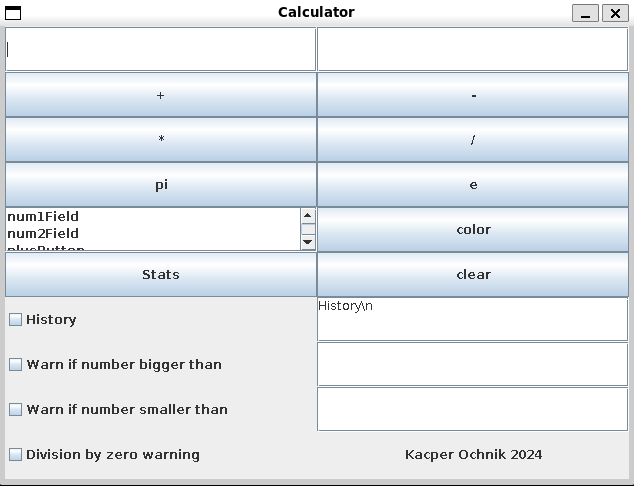
\includegraphics[width=0.8\textwidth]{./img/ui.png}
    \caption{Interfejs użytkownika}
    \label{fig:ui}
\end{figure}


\section*{3. Komponenty – Opis}

\subsection*{3.1. Math}

Moduł Math zawiera funkcje matematyczne, które są wykorzystywane przez kalkulator.
Zawiera również funkcje do serializacji danych.

\subsection*{3.2. Calculator}

Moduł Calculator zawiera interfejs użytkownika do kalkulatora.
Zawiera również funkcje do serializacji danych.

\subsection*{3.3. Stats}

Moduł Stats zawiera dane statystyczne kalkulatora oraz funkcje do ich wyświetlania.
Zawiera również funkcje do serializacji danych.

\newpage
\section*{4. Zmienne Prywatne i Ich Znaczenie}

\subsection*{4.1. Math}

\begin{itemize}
    \item private double a - pierwsza liczba
    \item private double b - druga liczba
    \item private boolean divisionByZeroWarning - zmienna logiczna, która określa czy wyświetlić ostrzeżenie o dzieleniu przez zero
    \item private boolean warnIfNumberBiggerThan - zmienna logiczna, która określa czy wyświetlić ostrzeżenie o przekroczeniu zakresu
    \item private boolean warnIfNumberSmallerThan - zmienna logiczna, która określa czy wyświetlić ostrzeżenie o przekroczeniu zakresu
    \item private boolean isVerbose - zmienna logiczna, która określa czy wyświetlić dodatkowe informacje
    \item private double warningNumberBig - górny zakres ostrzeżenia
    \item private double warningNumberSmall - dolny zakres ostrzeżenia
\end{itemize}

\subsection*{4.2. Calculator}

Kalkulator przechowuje w swoich prywatnych polach elementy UI.
    
\subsection*{4.3. Stats}

Komponent stats przechowuje przeróżne statystyki w prywatnych zmiennych oraz
elementy UI.

\begin{itemize}
    \item private static double largestNumber - największy wynik
    \item private static double smallestNumber - najmniejszy wynik
    \item private static double divisionsByZero - ilość dzielen przez zero
    \item private static double additions - ilość dodawań
    \item private static double subtractions - ilość odejmowań
    \item private static double multiplications - ilość mnożeń
    \item private static double divisions - ilość dzielen
    \item private static double pi - ile razy użyta została stała pi
    \item private static double e - ile razy użyta została stała e
    \item private static double startTime - czas rozpoczęcia działania kalkulatora
\end{itemize}

\section*{5. Funkcje Dostępowe do Zmiennych Prywatnych}

Komponenty posiadają funkcje dostępowe do wybranych zmiennych prywatnych które mają być udostępnione innym komponentom.

\section*{6. Przykłady Wywołań Setterów/Getterów Komponentu}

Przykładowe wywołania getterów i setterów można znaleźć poniżej:

\begin{verbatim}
    Math.setA(num2);
    Math.setB(num1);
    Math.div();
    double result = Math.getResult();
\end{verbatim}

\section*{7. Serializacja}

Komponent obsługuje serializację danych, co umożliwia zapis historii kalkulatora do pliku.
Serializacja danych jest również wykorzystywana do odczytu tekstów wyświetlanych w UI z pliku xml.
W ten sposób można łatwo zmieniać tekst wyświetlany w UI bez konieczności modyfikowania kodu.

\section*{8. Cechy Komponentu plus Fragmenty Kodu}

Komponent Math posiada funkcje do dodawania, odejmowania, mnożenia i dzielenia. Poniżej fragment kodu operacji dodawania:

\begin{verbatim}
    public static void add() {
        result = a + b;
        checkWarnings(result);
        verbose(a, b, '+', result);
    }
\end{verbatim}
Posiada on również opcje personalizacji np. możemy włączyć słowne wypisywanie wyników:

\begin{verbatim}
    public static void setVerbose(boolean bool) {
        isVerbose = bool;
    }

    public static void verbose(double a, double b, char operator, double result) {
        if (isVerbose) {
            System.out.println(a + " " + operator + " " + b + " = " + result);
        }
    }
\end{verbatim}

\section*{9. Testy Komponentu (Przypadki Testowe)}

Przeprowadzono testy jednostkowe, sprawdzające poprawność działania każdej z operacji kalkulatora.
Testy potwierdzają poprawność działania komponentu.
Przypadki testowe:

\begin{itemize}
    \item Dodawanie liczb dodatnich
    \item Dodawanie liczb ujemnych
    \item Dodawanie liczb zmiennoprzecinkowych
    \item Odejmowanie liczb dodatnich
    \item Odejmowanie liczb ujemnych
    \item Odejmowanie liczb zmiennoprzecinkowych
    \item Mnożenie liczb dodatnich
    \item Mnożenie liczb ujemnych
    \item Mnożenie liczb zmiennoprzecinkowych
    \item Dzielenie liczb dodatnich
    \item Dzielenie liczb ujemnych
    \item Dzielenie liczb zmiennoprzecinkowych
    \item Dzielenie przez zero
    \item Dzielenie przez zero z ostrzeżeniem
\end{itemize}
\newpage
\section*{10. Aplikacja Testująca Komponent}

Stworzono prostą aplikację testującą, która wykorzystuje komponent Math do przeprowadzania różnych operacji w celu przetestowania wszystkich przypadków testowych.

\begin{verbatim}
    public class Test {
        public static void main(String[] args) {
            System.out.println("");
            Math.setVerbose(true);
            Math.setDivisionByZeroWarning(true);
            Math.setWarnIfNumberBiggerThan(true, 10);
            Math.setWarnIfNumberSmallerThan(true, 0);
            Math.setA(0);
            Math.setB(0);
            Math.add();
            Math.sub();
            Math.div();
            Math.mul();
            Math.setA(-1);
            Math.setB(1);
            ...
        }
    }
\end{verbatim}

\section*{11. Przykład Wykorzystania Komponentu w Wybranej Aplikacji}

Komponent Math został użyty w aplikacji Kalkulator do obsługi obliczeń matematycznych oraz do dostępu do stałych matematycznych.

\section*{12. Wnioski}

Tworzenie aplikacji komponentowych jest bardzo intuicyjne, i przypomina budowanie klocków lego.
Każdy komponent jest odpowiedzialny za swoją funkcjonalność, co pozwala na łatwe rozszerzanie aplikacji.
Wadą jest konieczność tworzenia interfejsów, które są wymagane do komunikacji między komponentami.
Najwiekszą zaletą jest możliwość ponownego użycia kodu/komponentu w innej aplikacji.

\end{document}
